\documentclass[journal]{IEEEtran}
\usepackage{pifont}
\ifCLASSINFOpdf
\else
   \usepackage[dvips]{graphicx}
\fi
\usepackage{url}

\hyphenation{op-tical net-works semi-conduc-tor}

\usepackage{multirow}%表格
\usepackage{booktabs}

\usepackage{makecell}

\usepackage{graphicx}
\usepackage{amsmath}
\usepackage{bm}
\begin{document}

\title{A novel lightweight object detection architecture for helmet-wearing}

\author{Qi He, %\IEEEmembership{Fellow, IEEE}, 
Hao Shen, and Yang Jin %\IEEEmembership{Member, IEEE}
\thanks{This paragraph of the first footnote will contain the date on which you submitted your paper for review. 
The State Key Laboratory of Media Convergence and Communication sopports this work.
}
%\thanks{The next  few %paragraphs  should co ntain %the authors' current %affiliations, including %current address and e-mail. %For example, F. A. Author %is with the National %Institute of Standards and %Technology, Boulder, CO %80305 USA (e-mail: %autho the boulder.nist.gov).}
\thanks{Qi He, Hao Shen, Yang Jin are with the State Key Laboratory of Media Convergence and Communication, Communication University of China, Beijing, 100024, China(e-mail: shenhao@cuc.edu.cn; heqi654321@126.com).}}

\markboth{
}
{Shell \MakeLowercase{\textit{et al.}}: Bare Demo of IEEEtran.cls for IEEE Journals}
\maketitle

\begin{abstract}
Object detection is widely used in various fields. It has received special attention from researchers in academia and industry. In this paper, we design a novel lightweight safety helmet-wearing detection architecture based on the YOLOV4. Our work has three main contributions. Firstly, we adopt MobileNet as a backbone feature extraction network in the proposed model, which has fewer parameters than the original model. Secondly, our architecture uses Depthwise Separable Convolution to reduce the number of parameters. Moreover, we add an attention mechanism to MobileNet to improve the model's performance. Finally, experimental results demonstrate the effectiveness of our proposed methods.
\end{abstract}

\begin{IEEEkeywords}
object detection,  helmet-wearing
detection, attention mechanism, YOLOV4
\end{IEEEkeywords}


\IEEEpeerreviewmaketitle



\section{Introduction}

\IEEEPARstart{I}{n} the construction and manufacturing industries, there are often many security risks that threaten the personal safety of employees. A safety helmet protects personnel's heads in complex construction and manufacturing production environments. However, in China, due to the considerable mobility of construction personnel, lack of safety awareness, and inadequate supervision of personnel, it is a significant safety risk not in wearing safety helmets in real work.
Accordingly, helmet-wearing supervision is a vital link in risky operating environments. However, the traditional way of relying on manual supervision has many shortcomings, such as limited management scope, inability to monitor the whole field, and poor timeliness.

In recent years, convolutional neural networks (CNN) have widely used in deep learning tasks. It shows outstanding performance in image classification and recognition.
With the improvement of the computing power of the computer graphics processing unit(GPU), the performance of the object detection model improves rapidly. Object detection has become one of the most challenging problems in computer vision because different objects have different appearances, shapes, and postures and are affected by lighting, occlusion, and other factors.

Therefore, the helmet-wearing monitoring method based on object detection has been paid special attention by researchers from industry and academia to solve those issues.

Object detection can be divided into two stages and a single-stage framework. The two-stage target detection algorithm is parted into two steps: Firstly, extract candidate regions and then classify them, such as R-CNN[1], FastR-CNN [2], and FasterR-CNN[3]. Unlike the two-stage target detection algorithm, the single-stage target detection algorithm is simple in structure and fast in speed. It can directly identify the category of objects by extracting features in the network, such as the single-stage multi-box Detector (SSD)[4]  and the You Only Look Only (YOLO) [5] series networks. 

 Compared with other target detection networks, the improved methods based on the YOLO series network have  more extensively applied in various aspects. Helmet-wearing detection is a typical target detection problem. Shanshan Huang et al.[6] introduced an automatic safety helmet detection model using an attention mechanism. In 2022 year, Lixia Deng et al.[7] designed a lightweight and mini YOLOV3 object detection model for safety helmet detection. This method has obvious advantages in detection efficiency and calculation cost compared to other methods. This paper explores a safety helmet-wearing detection architecture based on the YOLOV4[8]. The significant contributions of this letter are summarized
as follows:
\begin{figure*}
\centerline{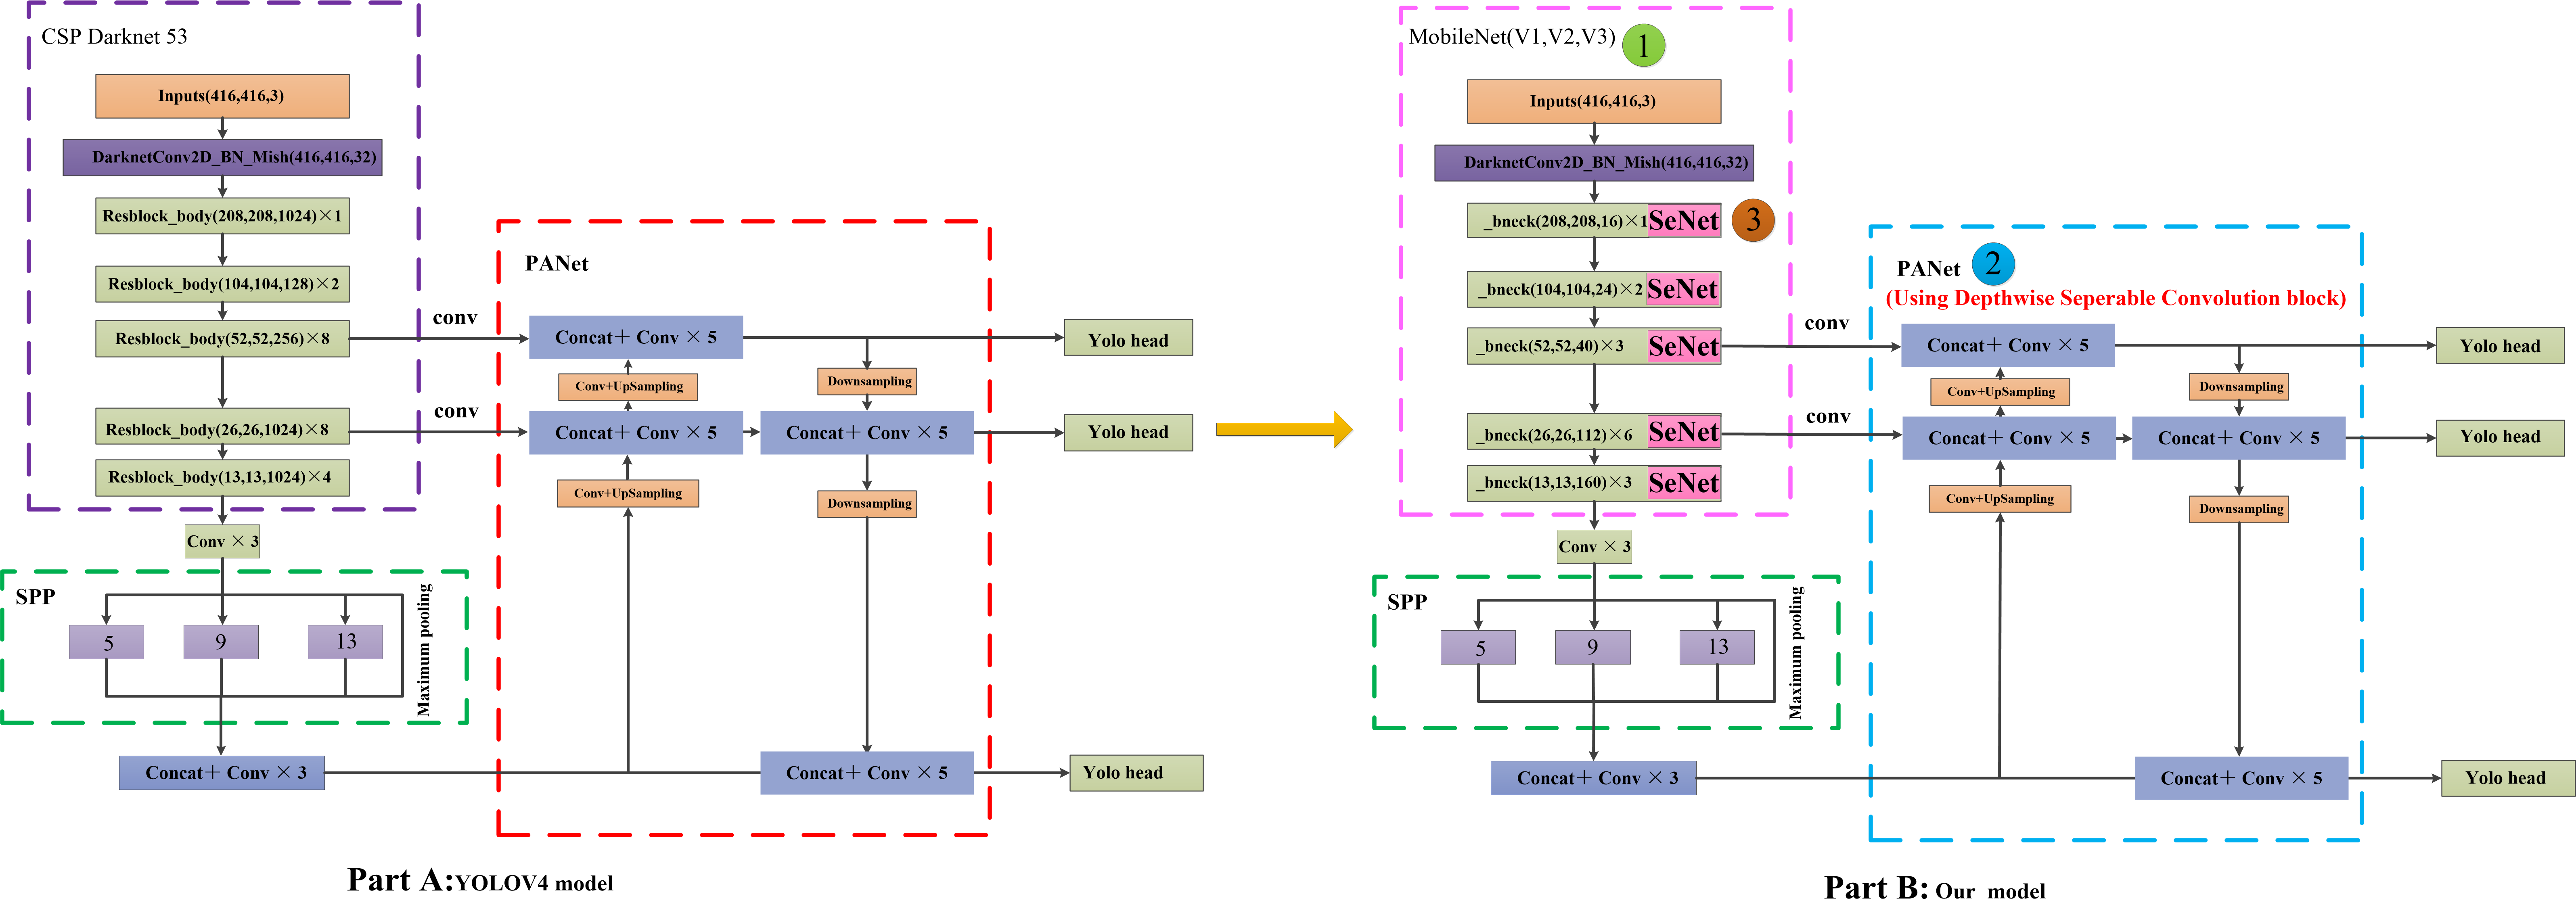
\includegraphics[width=2\columnwidth]{QiHe1.png}}
\caption{Our proposed helmet-wearing
detection architecture(Part B of this Figure). Part A of this Figure is the YOLOV4 model. The numbers labels (1, 2, 3) are the differences between Part A and B. 1: The lightweight MobileNet(V1, V2, V3) network replaces the backbone CSPDarknet53 in YOLOV4. 2: In the Path Aggregation Network(PANet) part, the Depth Separable Convolution instead of ordinary convolution to reduce the number of parameters. 3: There use the attention mechanism is used.}
\end{figure*}
\begin{enumerate}[]
\item The backbone feature extraction network CSPDarknet53 in YOLOV4 is replaced by a lightweight MobileNet(V1, V2, V3)network[9][10][11].

\item In Path Aggregation Network(PANet), by replacing ordinary convolution with Depthwise Separable Convolution, the parameters of convolution can be greatly reduced to achieve the goal of a lightweight model.
\item The attention mechanism module called Squeeze-and-Excitation Networks(SENet)[11] is added in MobileNet to enhance the feature extraction capability of the backbone network.
\end{enumerate}

Our improved methods have been applied to helmet-wearing
detection. The experimental results show that those methods
(especially method five and method seven)significantly reduce
the number of parameters and calculations, which is of great
significance for the intelligent detection of helmet-wearing.

%Our improved methods have been applied %to helmet-wearing detection.
 %The experimental results show that %those methods (especially method five %and method seven)significantly reduce %the number of parameters and %calculations, which is of great %significance for the intelligent %detection of helmet-wearing.
\section{APPROACHES}
In this section, we will describe our approaches. The overall pipeline of our system is shown in Fig.1(Part B).
\subsection{YOLOV4}
YOLOV4[8] is a single-stage target detection algorithm, which is faster and more accurate than previous versions. Fig.1(Part A) shows the pipeline of YOLOV4. The YOLOV4 network structure  composed mainly of the CSPDarknet53 backbone feature extraction module, Spatial Pyramid Pooling(SPP) module, PANet feature fusion module, and YoloHead classifier. The backbone network of YOLOV4 adopts a CSPDarknet53 network consisting of several residual convolution blocks. Input characteristics are processed using the SPP module's four maximum pooling layers of different sizes. The SPP structure can effectively increase the receptive field. Then the 64×64, 32×32, and 16×16 feature maps connected to the PANet feature fusion module, respectively. After the PANet module achieves bottom-up layer-by-layer sampling and feature fusion, and it will perform feature extraction from top to bottom.  
This repeated feature extraction gives the three different scale feature layers  better expression effects.
Then, the PANet module input feature maps into three YoloHead classifiers for classification, and the detection results are obtained.

 Compared to previous YOLO versions, YOLOV4 dramatically increases the amount of computing required for the model while improving performance. Therefore, to reduce the cost, we will optimize the YOLOV4 network to build a smaller, faster, and more applicable target detection network in real scenarios.
\subsection{Our methods}
Part B of Fig.1 shows our improved model. The numbers labels (1, 2,
3) are the differences between Part A and B. 1: The lightweight MobileNet(V1, V2, V3) network replaces the backbone CSPDarknet53 in YOLOV4. 2: In
the Path Aggregation Network(PANet) part, the Depth Separable Convolution instead of ordinary convolution to reduce the number of parameters. 3: There use the attention mechanism.

\subsubsection{MobileNet}
In recent years, Researchers have combined object detection models with mobile devices to develop algorithms with practical significance. In 2017, Google proposed the MobileNetV1[9] algorithm, a convolutional neural network model for mobile devices. The MobileNetV2[10] network, proposed by the google team in 2018, offers higher accuracy and smaller models than the MobileNetV1. In 2019, this team proposed a more advanced version of the MobileNetV3 model[11].
 In the MobileNetV3 network structure, There reduces the number of parameters and computation of the model,using the Depthwise Separable Convolution and SENet attention mechanism, which can improve the detection performance.
  \begin{figure}
\centerline{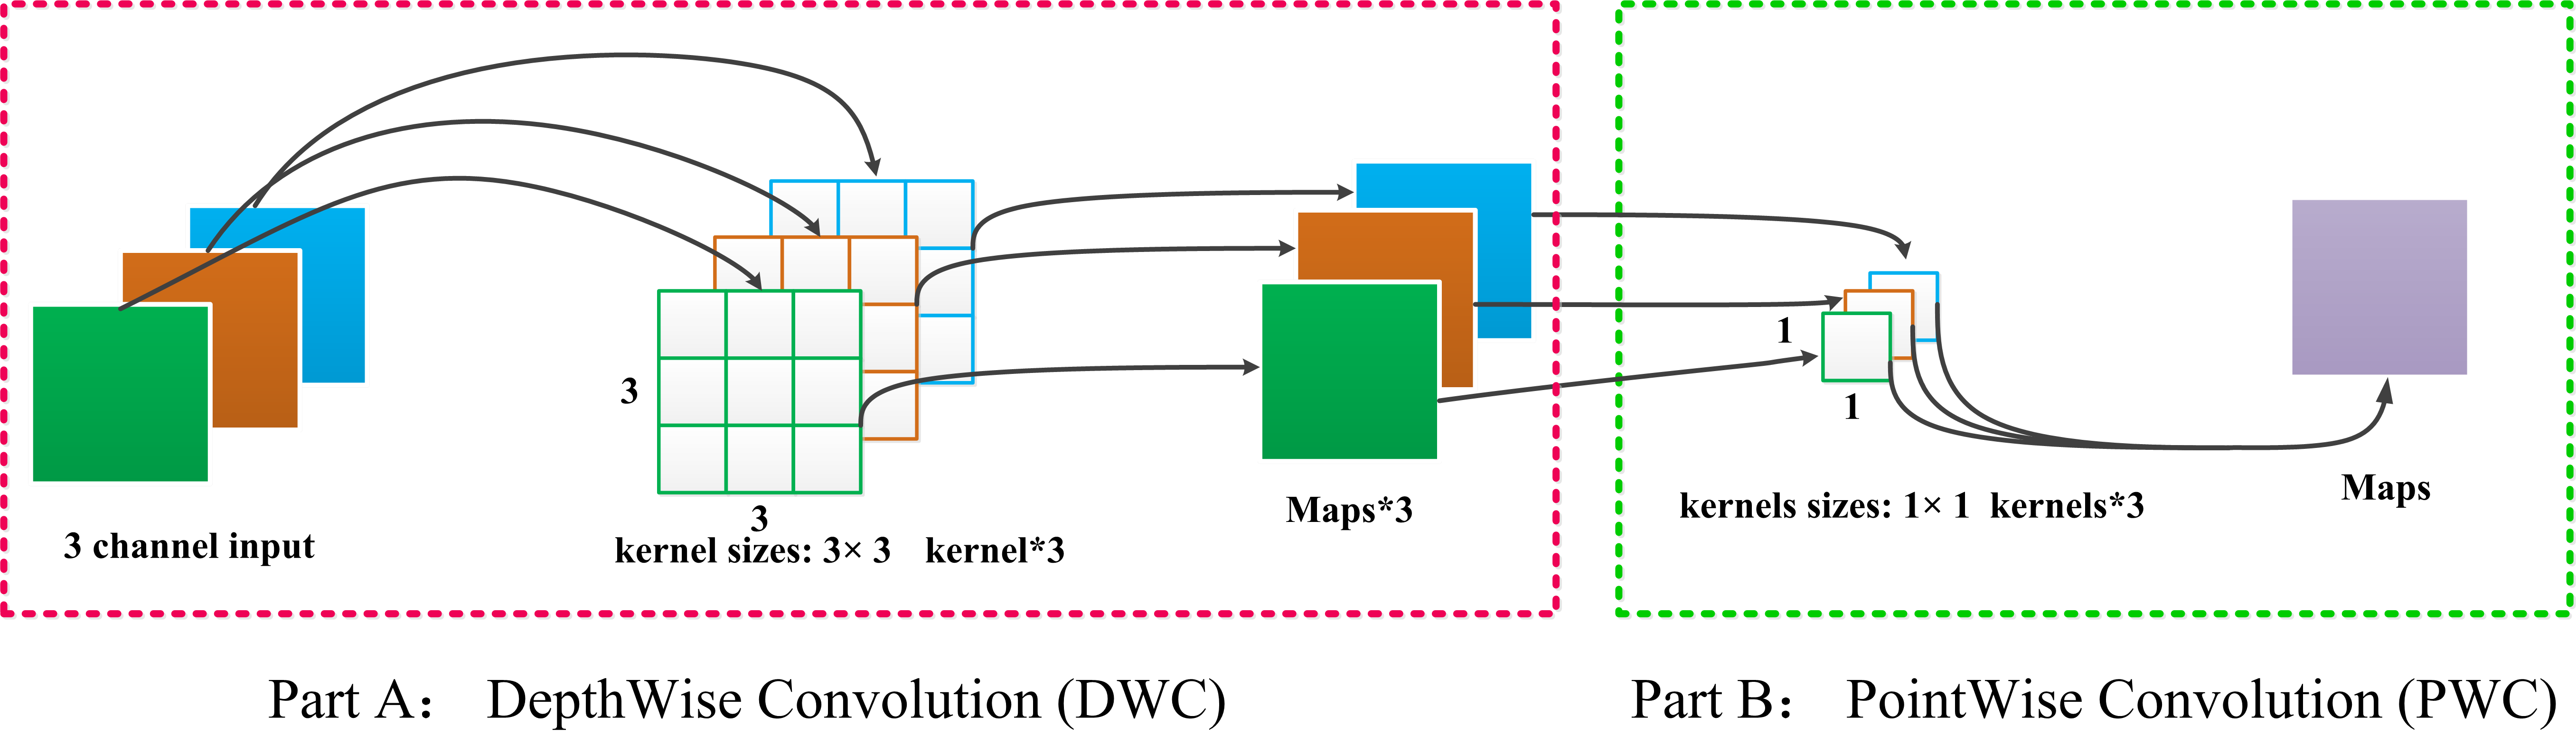
\includegraphics[width=0.9\columnwidth]{QiHe2.png}}
\caption{Depthwise Separable 
Convolution. (Part A of this Figure)DepthWise Convolution (DWC): Convolving the three input channels obtains three feature maps. Then, (Part B of this Figure)PointWise
Convolution (PWC): Three feature maps use three 1×1 convolution kernels to generate a feature map.}
\end{figure}
\subsubsection{Depthwise Separable 
Convolution (DSC)}
DSC(As shown in Fig.2) can greatly reduce the number of parameters in the convolution process. It often uses in the construction of lightweight networks. With ordinary convolution, when the input channel is there and the size of the convolution kernel is 3, it takes three convolution kernels to make a feature map. Therefore, the parameter required to generate m feature maps is p1.
$p 1=3 \times 3 \times 3 \times m=27m$.
 DSC divides into DepthWise Convolution (DWC) and PointWise Convolution (PWC). 
(Part A of Fig.2)DepthWise Convolution (DWC): Convolving the three input channels to obtain three feature
maps. Then, (Part B of Fig.2)PointWise
Convolution (PWC): Three feature maps use three 1×1 convolution kernels to generate a feature map. The parameter required to generate m feature maps is p2.
$p2=3 \times 3 \times 3+1 \times 1 \times 3 \times m=27+3 m.$


When m$>$1, the number of parameters required using DSC, p2, is less than the number of parameters needed using standard convolution, p1.
Therefore, to reduce the computational amount of the network, the 3$\times$3 convolution is replaced by DSC in our methods.


\subsubsection{Queeze and Excitation Networks(SENet)[12]}
In recent years, the attention mechanism has made breakthroughs in image classification, object detection, and instance segmentation to help improve the performance of the model. In this paper, SENet(Fig.3) module is used in the backbone feature extraction network to improve the detection effect of the algorithm. The number 3 in Part B of Fig.1 adds SENet.
SENet enhances the network’s ability to extract useful information by obtaining the weight of each channel in the input feature layer. Firstly, carrying out compression operation. The feature layer of each
channel is transformed into concrete data using global average pooling.
Secondly, the full connection layer is used to predict the importance of each
channel and get the importance of different channels. Thirdly, the Sigmoid
function normalizes, making the weight value range between[0,1]. Then, this
obtained weight is multiplied by the original input feature layer to complete
the weighting work. The following formulas (1), (2), (3), and Fig.3 describe how SENet works.

\begin{equation}
z=\frac{1}{W \times H} \sum_{i=1}^{W} \sum_{j=1}^{H} u_{c}(i, j)
\end{equation}
\begin{equation}
s=\sigma\left(w_{2} \delta\left(w_{1} z\right)\right)
\end{equation}
\begin{equation}
x_{c}=s_{c} \otimes u_{c}(i, j)
\end{equation}

z is the weight obtained by the compressed channel. $u_{c}$ represents the corresponding channel. $c$ is the channel. $i, j $\in \mathbb{R}$. ${H, W}:$ represents the height and width of the feature map, respectively. $\delta$ is the activation function ReLU.
$w_{1}$ and $w_{2}$ are full connection operation weights.
$\sigma$ is the normalized function Sigmoid.
$\otimes$ is the multiplication of elements one by one.
$s$ is the obtained weight.
$s_{c}$ is the obtained weight of the corresponding channel.
$x_{c}$ is the final result.

In the next section, we will train our model and apply it to predict the wearing of safety helmets in real work scenarios.
 
 \begin{figure}
\centerline{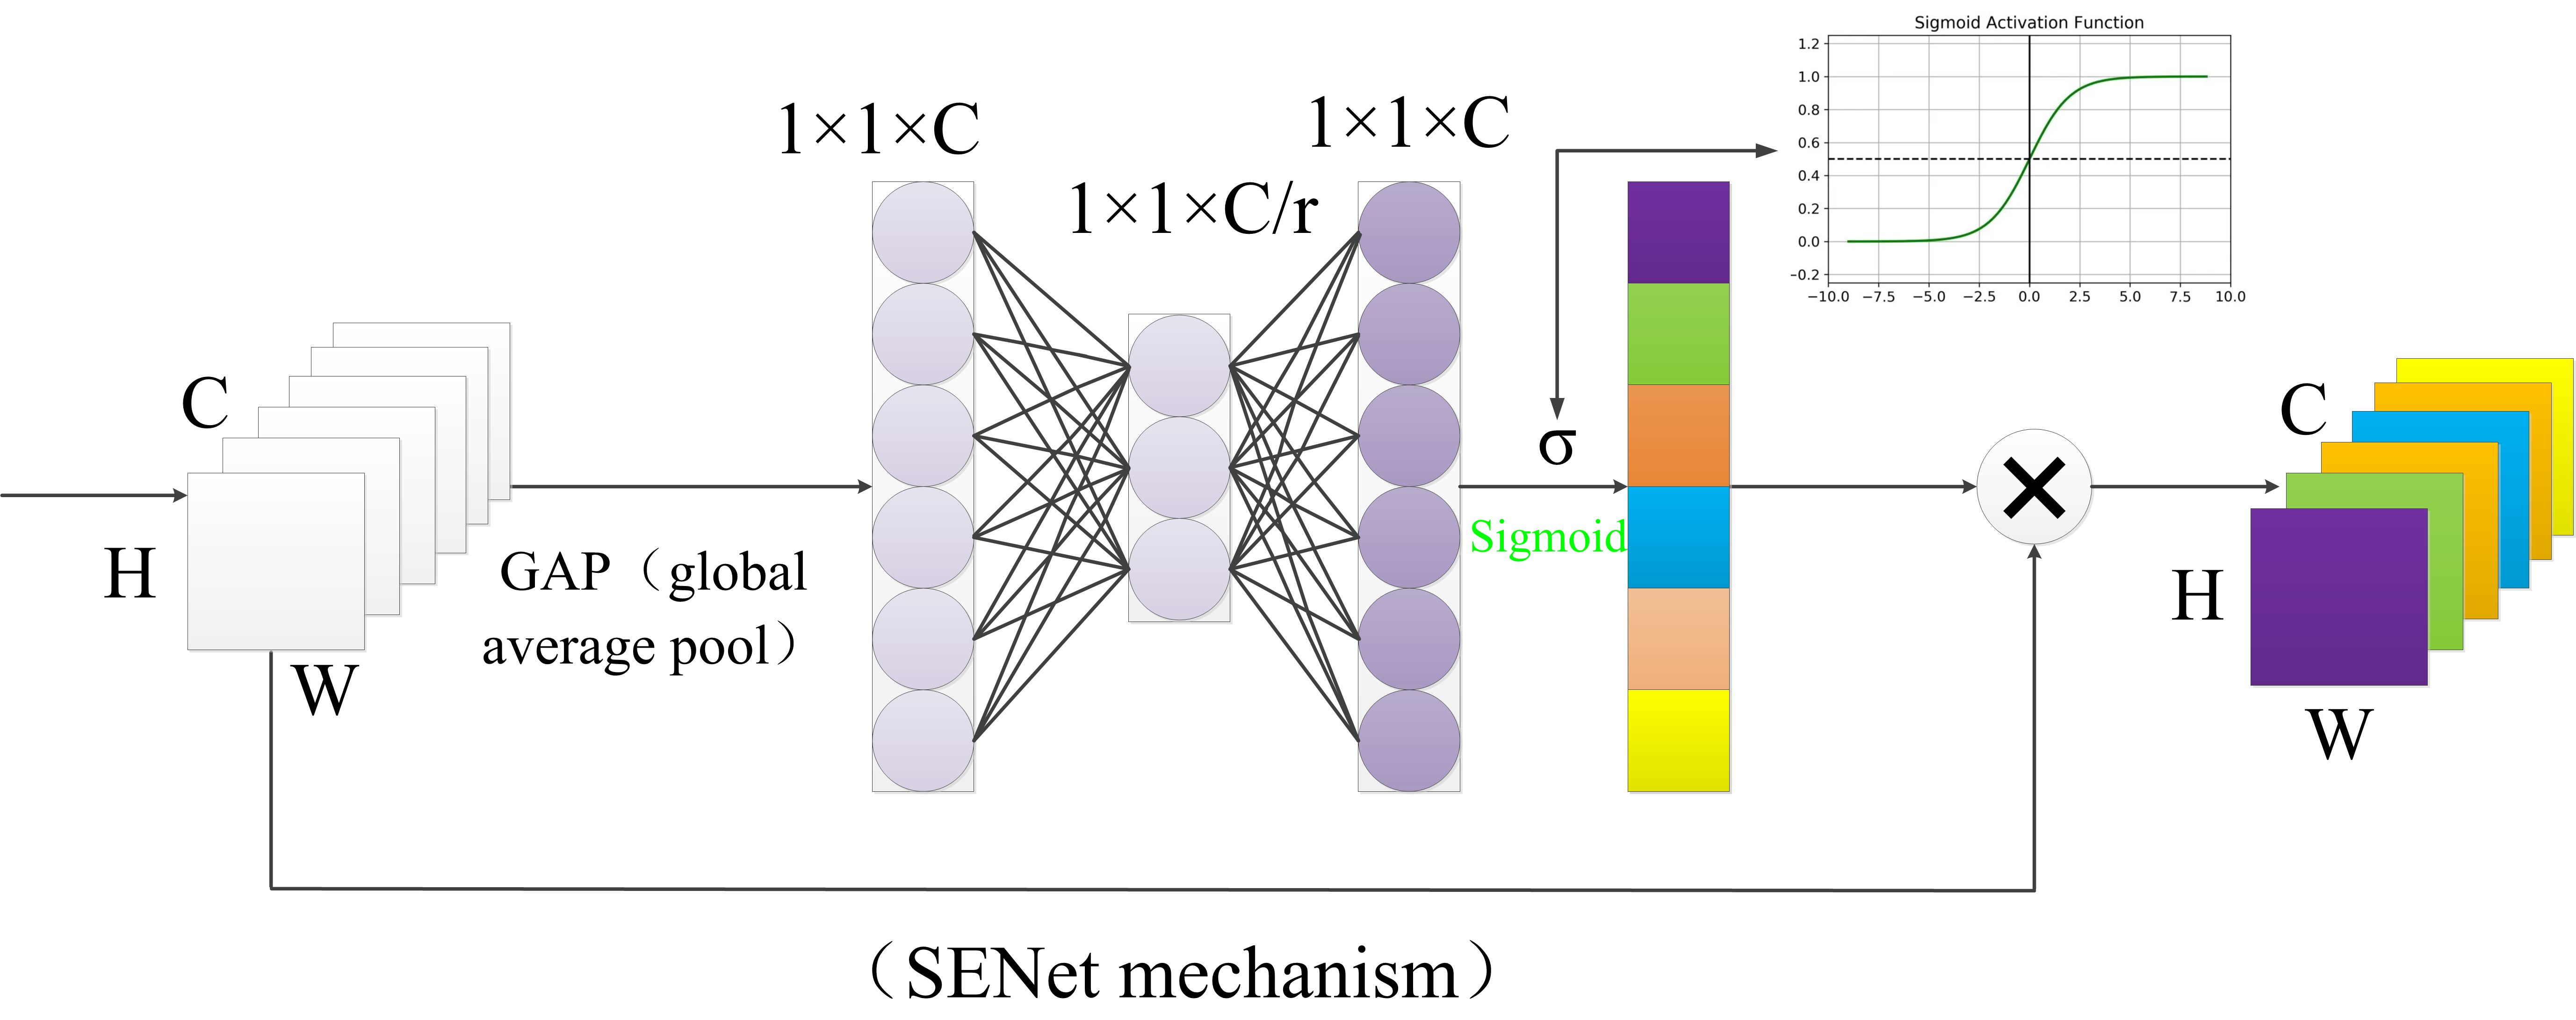
\includegraphics[width=\columnwidth]{QiHe3.png}}
\caption{Queeze and
Excitation Networks(SENet).In this Figure, C is the channel of the feature map. H, W:represents the height and width of the feature map, respectively. r=2. Firstly, carrying out compression operation. The feature layer of each the channel is transformed into concrete
data using global average pooling. Secondly, the full
connection layer is used to predict the importance of each
channel and get the importance of different channels. Thirdly, the Sigmoid function normalizes, making the weight value range between[0,1].
Then, this obtained weight is multiplied by the original input
feature layer to complete the weighting work.}
\end{figure}
\section{Experiments}

\subsection{Hardware and Software environment configuration}

\subsubsection{Hardware environment}{
$\bm{CPU: }$Intel (R) Core (TM) i7-1075H, $\bm{GPU: }$NVIDIA GeForce RTX 2080Ti, $\bm{RAM: }$16G.}
\subsubsection{Software environment}
{$\bm{OS: }$Window10, Tensorflow framework==1.13, $\bm{cuda :}$10.0, $\bm{cudnn: }$7.4.1.5.}


\subsection{Parameter setting}
In this experiment, the input image size is set to 416×416. The network's training divides into two phases, frozen and unfrozen. Firstly, the backbone feature extraction network is frozen. Init$_$Epoch$=$0; Freeze$_$Epoch$=$50; Freeze$_$batch$_$size$=$8. The learning rate is le-7; Secondly, unfreeze the backbone and train the entire network. UnFreeze$_$Epoch$=$400(The total epoch of the model is trained); The batch size at this stage is four, and the learning rate is le-2. Optimizer-Type='sgd', momentum parameter$=$0.937, weight-Decay=5e-4. The learning rate decline mode used $\bm{cos}$.

\subsection{Datasets}
Helmet wearing dataset derives from the network platform[13]. In the experiment, 10000 images are obtained using Data Augmentation such as rotation, cropping, translation, mirroring, adding noise, and changing brightness. The training set size is 8100, the validation set is 900, and the test set is 1000.

\subsection{Experimental evaluation method}
The following formulas (4), (5), (7), and (8) use to evaluate the training models.
 Precision(P) is the proportion of predicted true positive samples in all predicted positive samples. Recall(R) is the proportion of predicted true positive samples in all true positive samples. The value of Average Precision(AP) is the area of the graph enclosed by the Precision-Recall(PR) curve and the X-axis and Y-axis. It generally calculates using the integral method. The mAP is the average of the AP values for each detected class. The F1 value is the harmonic average of the Precision and Recall.
\begin{table*}
\begin{center}

\caption{Performance comparison between our improved methods and YOLOV4}
\label{table}
\small
\setlength{\tabcolsep}{4.5pt}
\centering
%\setlength{\tabcolsep}{2mm}
{
\begin{tabular}{cccccccccc}
\hline
\toprule[1.1pt]
Methods&Backbone&DSC$^{\mathrm{a}}$&SENet&\makecell{Precision\\@$^{\mathrm{c}}$0.5(\%)}&\makecell{Recall\\@0.5(\%)}& \makecell{mAP\\@0.5(\%)}&\makecell{F1\\@0.5(\%)}& Total params& Total GFLOPS$^{\mathrm{b}}$\\
\hline
\toprule[0.5pt]
YOLOV4& CSPdarknet53&\ding{56}&\ding{56}&
\bm{96.20}&90.45&\bm{95.38}& 93& 63,384,157 & 58.903G \\

Improved method 1& CSPdarknet53&\ding{52}&\ding{56}&
95.51&\bm{90.50}&95.20&\bm{93}&35,752,342 & 40.657G \\

Improved method 2& MobileNetV1&\ding{56}&\ding{56}&
 95.15& 85.70& 93.43& 90 &39,535,094 & 27.635G\\

Improved method 3& MobileNetV1&\ding{52}&\ding{56}&
 94.45& 82.67& 92.63 & 88 & 12,328,694 & 9.965G\\

Improved method 4& MobileNetV2&\ding{56}&\ding{56}&
 95.41& 83.38& 92.90 & 89 &37,653,878 & 25.247\\

Improved method 5& MobileNetV2&\ding{52}&\ding{56}&
 94.43& 81.42& 91.48& 87 &\bm{10,447,478} & 7.577G\\

Improved method 6& MobileNetV3&\ding{56}&\ding{52}&
95.02& 84.42& 92.80& 89 &38,572,726 & 24.694\\

Improved method 7& MobileNetV3&\ding{52}&\ding{52}&
 94.51& 79.84& 91.06& 87 &11,366,326 & \bm{7.023G}\\

\bottomrule[1.1pt]

%\multicolumn{3}{p{55pt}}{}
\end{tabular}}
\label{tab1}
\end{center}
\begin{tablenotes}
   \footnotesize
      \item [1] \quad\quad$^{\mathrm{a}}$$\bm{DSC}$-Depthwise Separable Convolution: In the Path Aggregation Network(PANet) part, the depth separable convolution instead of standard convolution.
      \quad\item[2] \quad\quad$^{\mathrm{b}}$$\bm{GFLOPS}$: Giga Floating-point Operations Per Second.
      \quad\item[3] \quad\quad$^{\mathrm{c}}$@$:$ The number after "@" represents the threshold of Intersection over Union(IOU).
      
\end{tablenotes}
\end{table*}

\begin{center}
\begin{equation}
Precision=\frac{T P}{T P+F P}
\end{equation}
\end{center}
\begin{center}
\begin{equation}
Recall=\frac{T P}{T P+F N} 
\end{equation}
\end{center}

   Where, TP is True Positive. TN is a True Negative. FP is False Positive. FN is False Negative.
\begin{center}
\begin{equation}
A P=\int_{0}^{1} P(r) d r
\end{equation}
\end{center}

\begin{center}
\begin{equation}
mAP=\frac{\sum_{i=1}^{K} A P_{i}}{K}
\end{equation}
\end{center}

   Where, K is the number of detected categories,  $AP_{i}$ represents i-th category's the value of Average Precision(AP), and the number of detection categories in this experiment is 1.
\begin{equation}
F_{1}=2 \cdot \frac{\text { Precision } \cdot \text { Recall }}{\text { Precision }+\text { Recall }} 
\end{equation}


\subsection{Experimental results and analysis}
Based on YOLOV4, we propose seven improved methods (1, 2, 3, 4, 5, 6, 7). To verify the effectiveness of the proposed improved algorithms, we conducted comparative experiments on the test set.
The comparisons mainly include the selection of different backbone feature extraction networks, whether to use Depthwise Separable Convolution, and whether to use the SENet attention mechanism.


The experimental results of helmet-wearing detection are listed in Table 1. Fig.4 shows the comparison results of calculation cost between our improved methods and YOLOV4. Furthermore, Fig.5 shows the comparative performance between our improved methods(5,7) and YOLOV4.

Our methods(3,5,7) aim to reduce the model's calculation cost while maintaining high detection quality.


In the improved method 1, Depth Separable Convolution is used. The parameters are reduced by 43.6\%, and the Giga Floating-point Operations Per Second(GFLOPS) is reduced by 30.9\% than the YOLOV4. The performance of the model is almost unchanged. The Recall is also 0.05\% higher than the original model. 

It can be seen from Table 1 and Fig.4 that the improved method 5 reduces the number of parameters by 83.5\% compared with the YOLOv4 algorithm. GFLOPS is reduced by 87.1\% than the YOLOV4.  

Parameter size, FLOPS of the improved
method 7 decreased by 82.1\% and 88.1\%  compared with the YOLOv4 algorithm.

The proposed improved method in this paper  effectively reduces the model's calculation cost while successfully ensuring the detection effect.


\begin{figure}[h]
\centerline{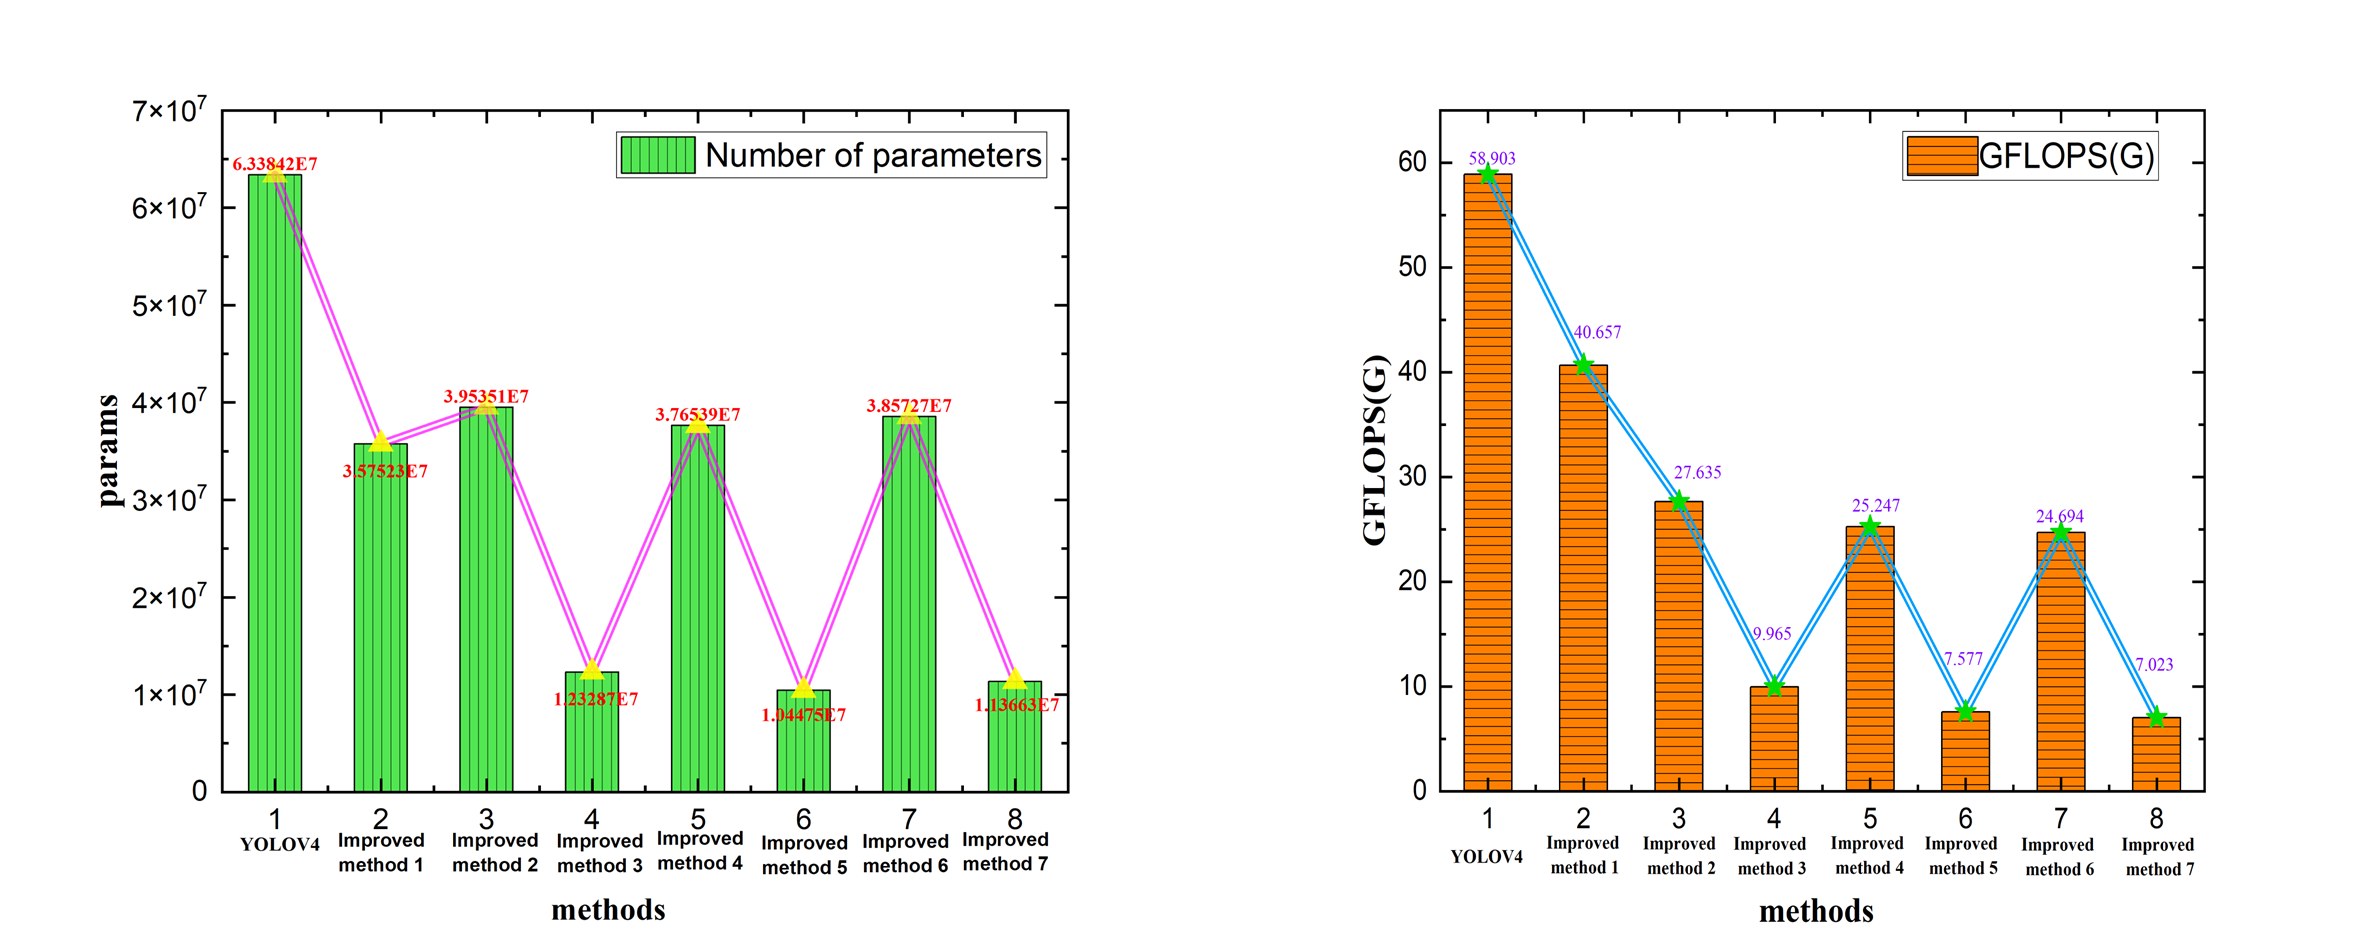
\includegraphics[width=1.1\columnwidth]{QiHe4.png}}
\caption{The number of parameters required by different methods(left Figure) and the Giga Floating-point Operations Per Second required for different methods(right Figure).}
\end{figure}

\begin{figure}[h]
\centerline{\includegraphics[width=1\columnwidth]{QiHe5.png}}

\caption{Performance comparison between YOLOV4 and our improved methods(5,7).}
\end{figure}
\section{Conclusion}
In this work, we propose a novel
helmet-wearing detection framework. Our improved seven methods adopt this more lightweight and straightforward structure. Experimental results show that our proposed model exhibit competitive performance. Undoubtedly, it is of great significance to practical application. Nevertheless, the algorithms in this paper still have room for performance improvement. We will leave it for our further work.

% the improved YOLOV4 algorithm is used to improve the defect detection of escalator steps under different actual backgrounds. Compared with the classic Mask RCNN and DeepLabv3+ image segmentation algorithms, the proposed algorithm has a higher accuracy in the escalator step defect detection, reaching 85\%, which is 12\% and 8\% higher than the previous year respectively. This algorithm is of great significance to practical application.
%\section*{References}
\begin{thebibliography}{1}
%\def\refname{}
\bibitem{}R. Girshick, J. Donahue, T. Darrell, J. Malik, “Rich feature hierarchies for accurate object detection and semantic segmentation,” in IEEE Conf. Comput. Vis. Pattern Recognit., 2014, pp. 580–587.

\bibitem{}R. Girshick, “Fast R-CNN,” in IEEE Int. Conf. Comput Vis., 2015, pp. 1440–1448.

\bibitem{}S. Ren, K. He, R. Girshick, J. Sun, “Faster R-CNN: Towards Real-Time Object Detection with Region Proposal Networks,” IEEE Trans. Pattern Anal. Mach. Intell., vol. 36, no. 6, pp. 1137-1149, Jun. 2017.


\bibitem{}W. Liu, D. Anguelov, D. Erhan, C. Szegedy, S. Reed, C.Y. Fu, A.C.
Berg, “SSD: Single shot multibox detector,” in Eur. Conf. Comput. Vis., 2016, pp. 21–37.
\bibitem{} J. Redmon, S. Divvala, R. Girshick, A. Farhadi, “You only look once: Unified, real-time object detection,”in IEEE Conf. Comput. Vis. Pattern Recognit., 2016, pp. 779–788.
\bibitem{} S. S. Huang, J. H Huang, and Y. Q Kong. “Attention Guided YOLOv3 for Wearing Safety Helmet Detection,”In 2020 the 6th Int. Conf. on Communica.Informat.Process., New York, NY, USA, 2021, pp. 65–69.
\bibitem{} Deng, L., Li, H., Liu, H. et al. “A lightweight YOLOv3 algorithm used for safety helmet detection,” Sci. Rep., vol.12, no. 1, pp.1-15, Jun. 2022.

\bibitem{} Bochkovskiy, A.,  C. Y. Wang, and  H. Liao. “YOLOv4: Optimal Speed and Accuracy of Object Detection,”arXiv:2004.10934.
\bibitem{}Howard, Andrew G. et al. “MobileNets: Efficient Convolutional Neural Networks for Mobile Vision Applications,” arXiv:1704.04861.
\bibitem{}M. Sandler, A. Howard, M. Zhu, A. Zhmoginov and L. C. Chen, “MobileNetV2: Inverted Residuals and Linear Bottlenecks,” in IEEE Conf. Comput. Vis. Pattern Recognit., 2018, pp. 4510-4520.
\bibitem{}A. Howard et al., “Searching for MobileNetV3,” in IEEE Int. Conf. Comput Vis., 2019, pp. 1314-1324.
\bibitem{}J. Hu, L. Shen, S. Albanie, G. Sun and E. Wu, “Squeeze-and-Excitation Networks,” in IEEE Trans. Pattern Anal. Mach. Intell., vol. 42, no. 8, pp. 2011-2023, Aug. 2020.
\bibitem{}Using Safety Helmet Detection Datasets in this letter. [Online]. Available: https://www.kaggle.com/datasets/andrewmvd/hard-hat-detection.
\end{thebibliography}

\end{document}
